\chapter{Dashboard Interface Design}
\label{app:interface}

This appendix records how the driver's dashboard on the Raspberry Pi~5 was redesigned between 11 and 12 October: the steps, the rules the design follows, and how each step was checked. The data path behind the pages is described in Section~\ref{sec:dashboard-page}. The redesign was deployed to the Pi~5 on 12 October (commit \texttt{5baa5f2}). \emph{It has not yet been used on the vehicle, and glance times have not been measured.}

\section{Starting point and constraints}

The inherited dashboard (Figure~\ref{fig:ui-before}) is the vacation-work teams' PySide6 application. It has eight pages: Driving, Analytics, Diagnostics, Navigation, Front camera, Sensors, Charging and Settings.

Every SW-7 change reaches it as a patch with an exact anchor, applied to a copy (\texttt{DashboardIntegration/tests/dashboard\_patches.py}), so the team's own copy is never edited. Each stage of the redesign has an environment switch that restores the previous look exactly, and a test checks that it does.

Four constraints shaped the design:
\begin{itemize}
\item it is read at a glance while driving, in sun and at night;
\item it is touched on a moving vehicle, possibly with gloves;
\item it must keep live data and simulated data visibly apart;
\item it must change only the presentation, never the telemetry, routing or sensor logic.
\end{itemize}

\begin{figure}[htbp]
\centering
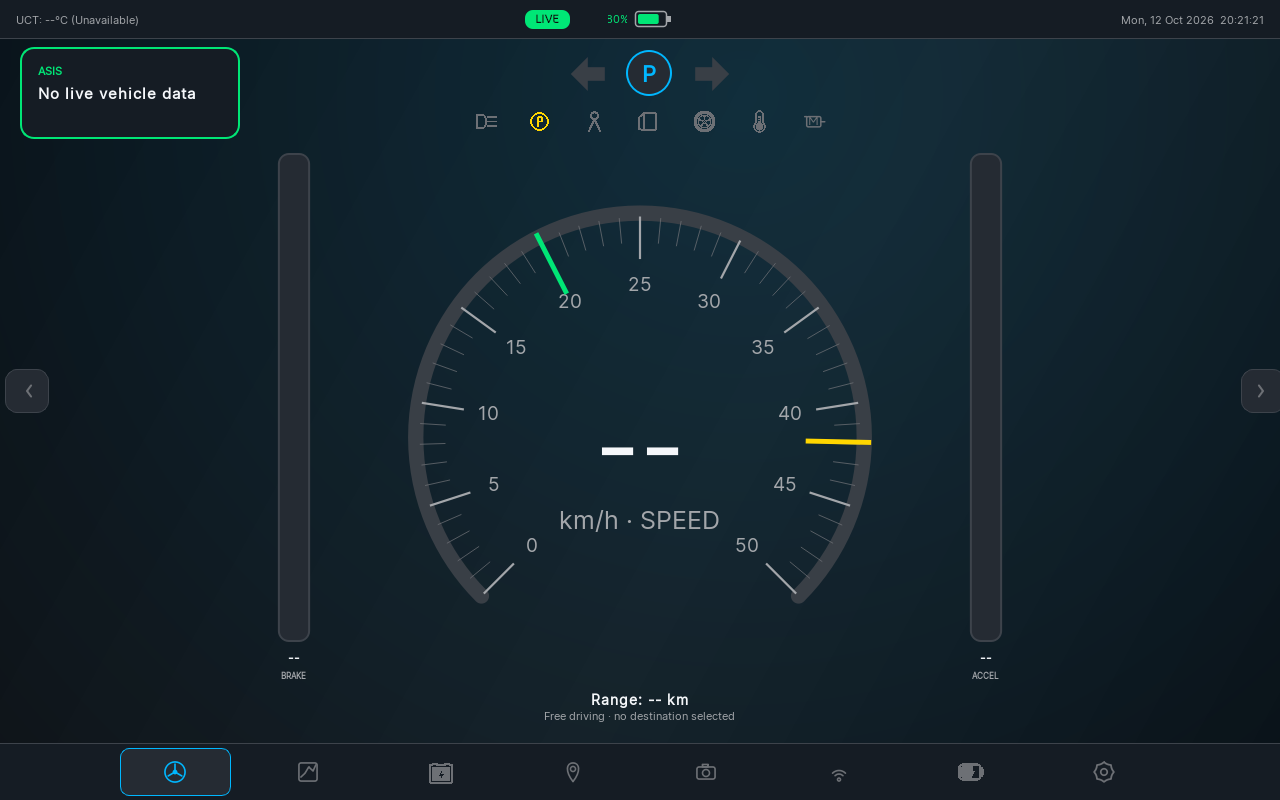
\includegraphics[width=0.7\textwidth]{figures/ui/ui_team_before.png}
\caption{The inherited Driving page, before the redesign (no live vehicle data).}
\label{fig:ui-before}
\end{figure}

\section{Design process}

The redesign was done in four steps. Each step was written as a brief in \texttt{Planning/} and checked by tests and screenshots before the next began.

\begin{enumerate}
\item \emph{Layout pass.} A page-by-page review set minimum sizes:
  \begin{itemize}
  \item 64\,px touch targets;
  \item driver-facing values of at least 32\,px;
  \item a 48\,px status bar with 16\,px text, against 38 and 11\,px before.
  \end{itemize}
  The pass also fixed real faults. The Charging page showed 79\% while the status bar showed 80\%, because one truncated and the other rounded.
\item \emph{Data ownership and page merge.} An audit found the same data shown in several places:
  \begin{itemize}
  \item battery percentage in seven places;
  \item link health on two pages;
  \item two different arrival estimates on the map at once;
  \item two unlabelled outside temperatures.
  \end{itemize}
  The student chose to keep the pages but remove the duplicates. Each value now has one home page and appears elsewhere only as a glance value that opens it. The Front camera and Sensors pages were merged into one page, Surroundings, leaving seven pages. Drive became the glance page, with tiles for the next turn, the surroundings and the range.
\item \emph{Paper theme.} The student supplied a reference with paper and ink, one terracotta colour for anything that can be tapped, and very large or very small type. Live weather (Open-Meteo) was added, along with a night variant that switches at sunset.
\item \emph{Refinement.} A second brief asked for restraint:
  \begin{itemize}
  \item IBM Plex Sans for the interface and Plex Mono for readings;
  \item fine borders and small radii in place of floating cards;
  \item a flat navigation bar;
  \item the weather inline in the status bar, with no box;
  \item status that never relies on colour alone;
  \item a dark mode designed in its own right;
  \item the team's battery animation kept, in the new colours.
  \end{itemize}
\end{enumerate}

\section{Design rules}

Table~\ref{tab:ui-rules} lists the rules the pages follow. Two are checked automatically over every page: no non-interactive element uses the tap colour, and every text size comes from the type scale.

\begin{table}[htbp]
\centering
\caption{Interface design rules and their reasons.}
\label{tab:ui-rules}
\small
\begin{tabular}{|p{3.6cm}|p{5.6cm}|p{5.2cm}|}
\hline
\textbf{Rule} & \textbf{Applied as} & \textbf{Reason} \\ \hline
One tap colour & Terracotta only on buttons, toggles, sliders, links and the selected page; checked over every page & The driver can tell what responds to touch without reading \\ \hline
Status not by colour alone & A word with every status mark, for example ``Left, close'' or ``Unavailable'' & Readable in glare and by drivers with colour-vision deficiency \\ \hline
Unavailable is not zero & ``--'' and ``Unavailable'' in muted grey, never 0 & A missing value must not look like a valid reading \\ \hline
Live against simulated & Source chip (LIVE, REPLAY, NO DATA, SIMULATED) and a strip on every page during a simulated drive & Simulated data must never be mistaken for the vehicle's \\ \hline
One hero value per page & Speed, odometer, nearest obstacle, battery, turn distance at 120 to 180\,px; the rest at 13, 16 or 22\,px & A clear hierarchy at a glance \\ \hline
Tabular figures & IBM Plex Mono for changing numbers & Values do not shift as their digit count changes \\ \hline
Touch targets & At least 64\,px & Use on a moving vehicle \\ \hline
One home per value & Other pages show a glance value that opens the home page & Removes duplicated and conflicting figures \\ \hline
Night variant & Charcoal surfaces, the same layout and tap colour, from sunset to sunrise & A white screen dazzles at night \\ \hline
\end{tabular}
\end{table}

\section{The pages}

Figures~\ref{fig:ui-drive} to~\ref{fig:ui-pages-b} show the deployed pages. The screenshots are from the test suite at the display's native 1280 by 800, with test data.

\begin{figure}[htbp]
\centering
\subfigure[Drive, day: speed, next turn, surroundings and range tiles; the weather inline at top left.]{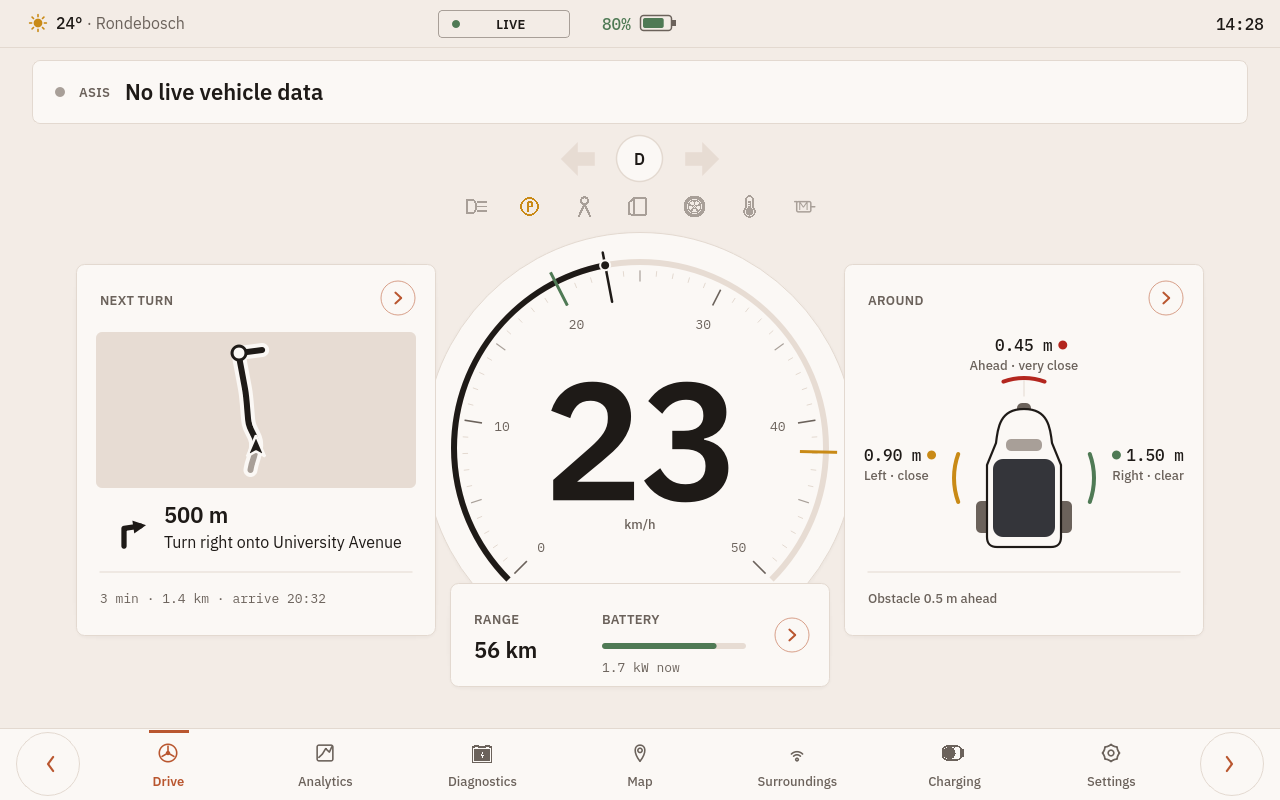
\includegraphics[width=0.48\textwidth]{figures/ui/ui_drive_day.png}}
\subfigure[Drive, night variant.]{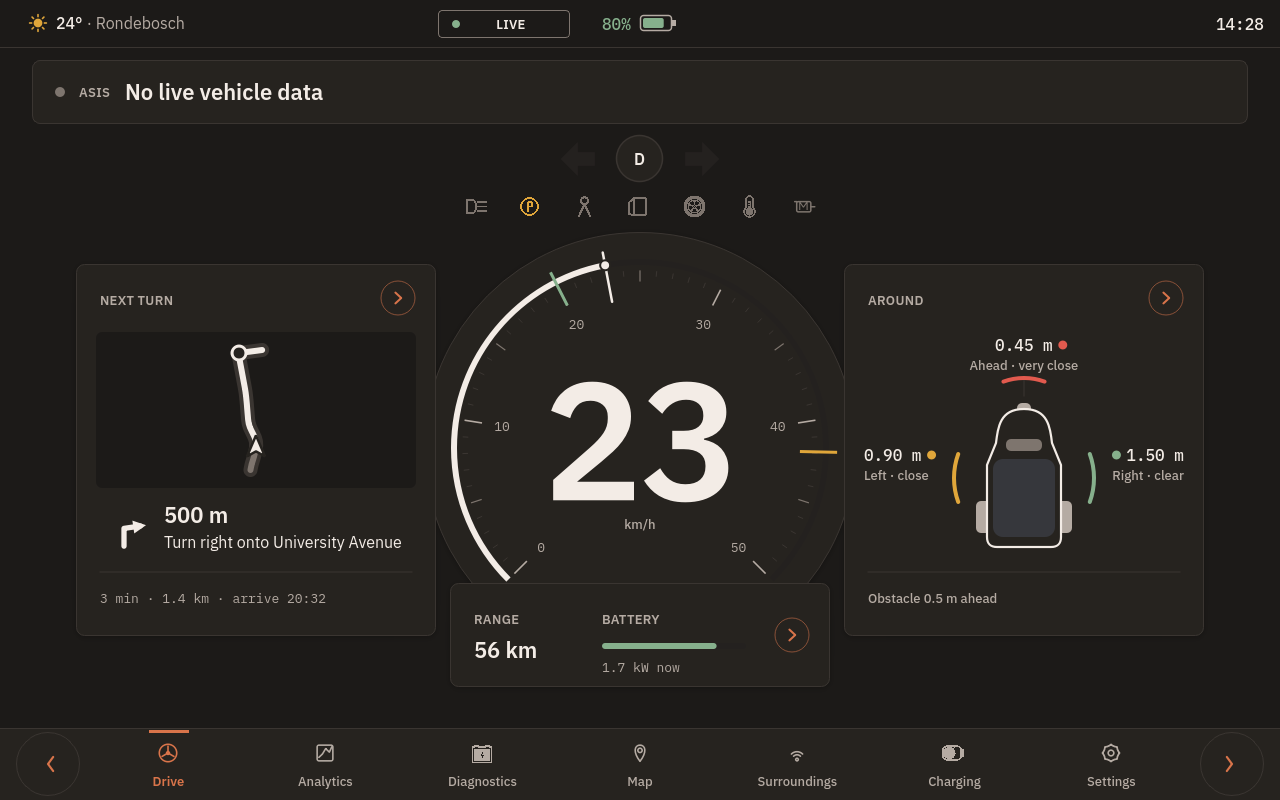
\includegraphics[width=0.48\textwidth]{figures/ui/ui_drive_night.png}}
\caption{The Drive page after the redesign.}
\label{fig:ui-drive}
\end{figure}

\begin{figure}[htbp]
\centering
\subfigure[Map: turn banner, single arrival bar, control column.]{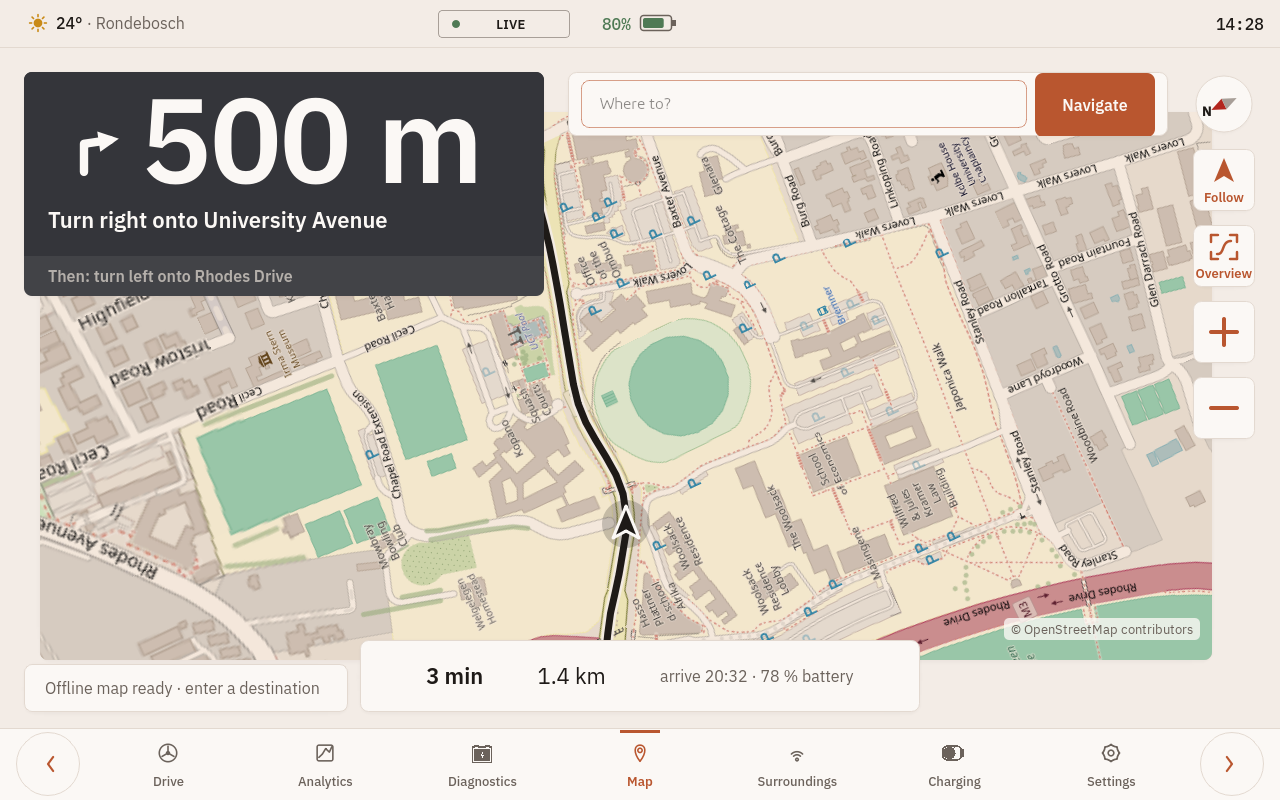
\includegraphics[width=0.48\textwidth]{figures/ui/ui_map.png}}
\subfigure[Surroundings: camera, the three ToF distances around the vehicle, one combined hazard list.]{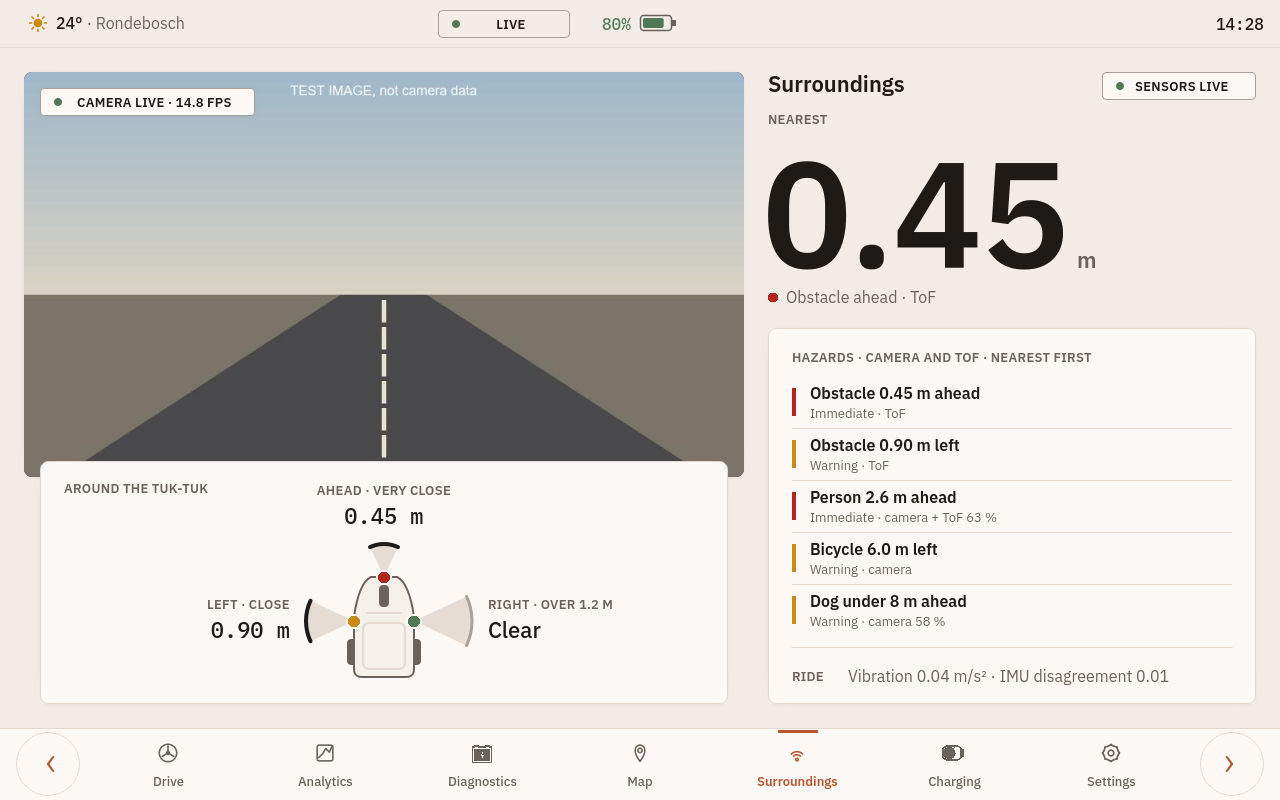
\includegraphics[width=0.48\textwidth]{figures/ui/ui_surroundings.png}}
\subfigure[Charging, with the team's battery animation restyled.]{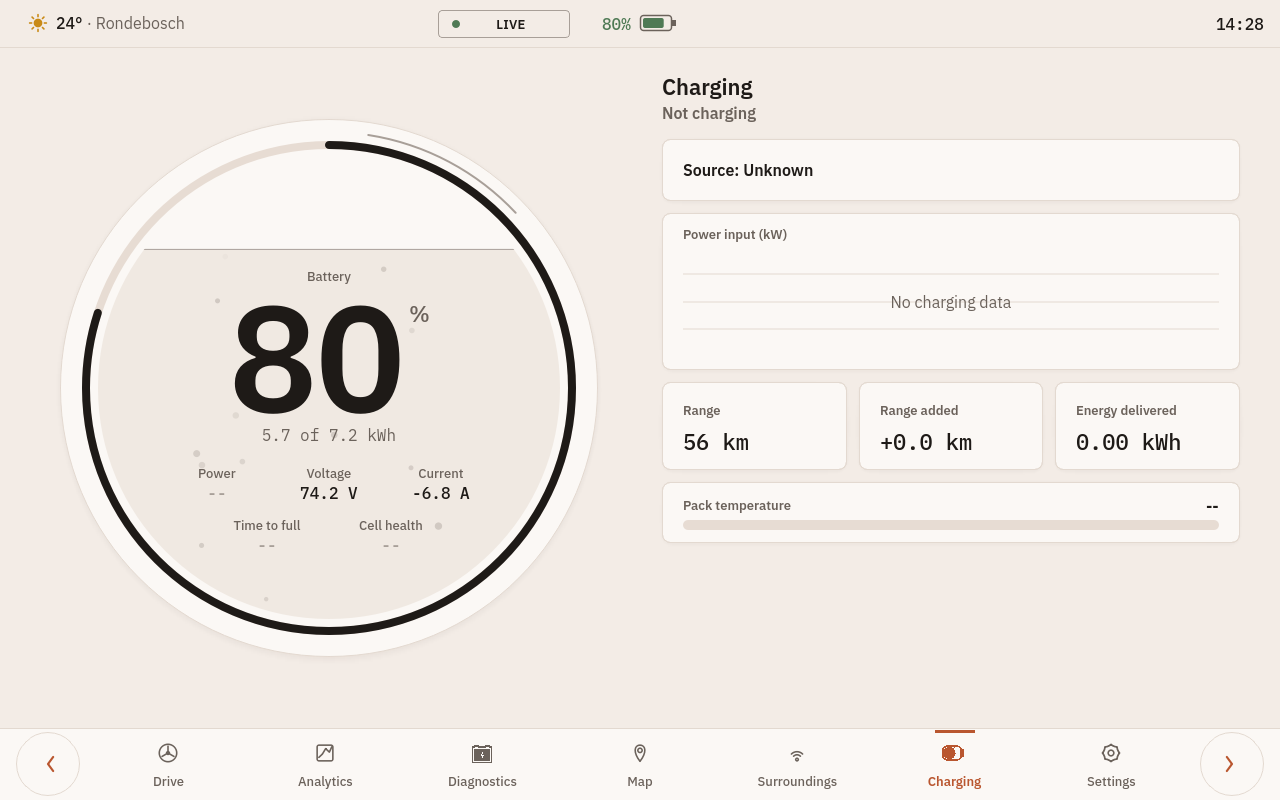
\includegraphics[width=0.48\textwidth]{figures/ui/ui_charging.png}}
\subfigure[Diagnostics: four groups; unavailable values in words.]{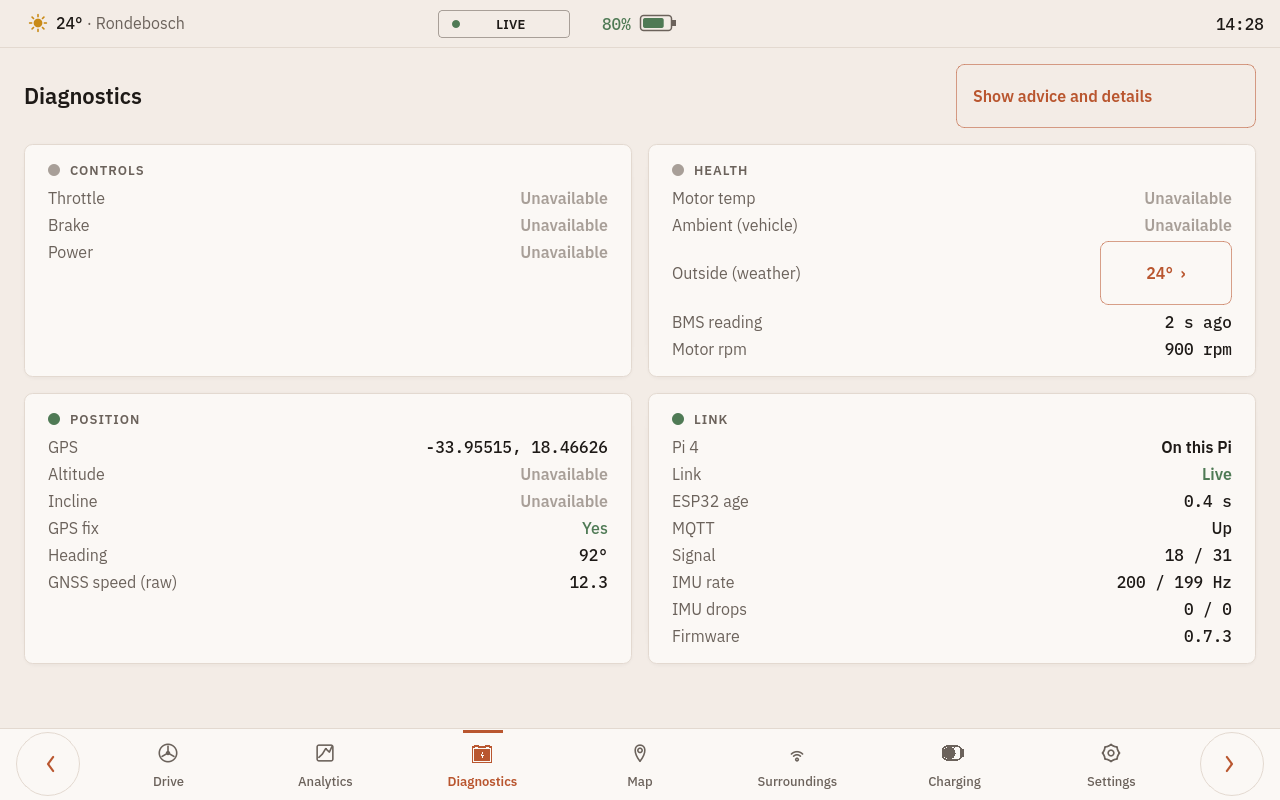
\includegraphics[width=0.48\textwidth]{figures/ui/ui_diagnostics.png}}
\caption{Map, Surroundings, Charging and Diagnostics pages.}
\label{fig:ui-pages-a}
\end{figure}

\begin{figure}[htbp]
\centering
\subfigure[Analytics: one value per card in a vertical carousel.]{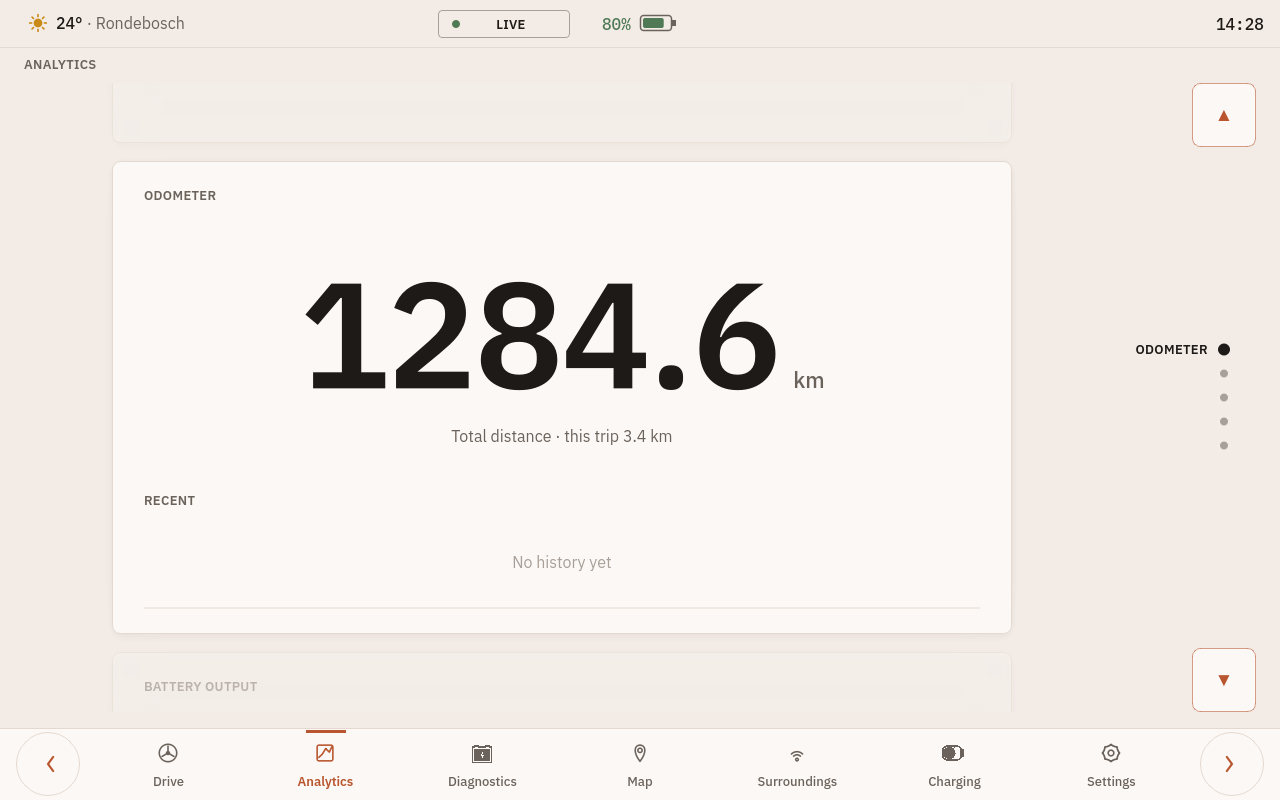
\includegraphics[width=0.48\textwidth]{figures/ui/ui_analytics.png}}
\subfigure[Settings, including the Auto, Day and Night look.]{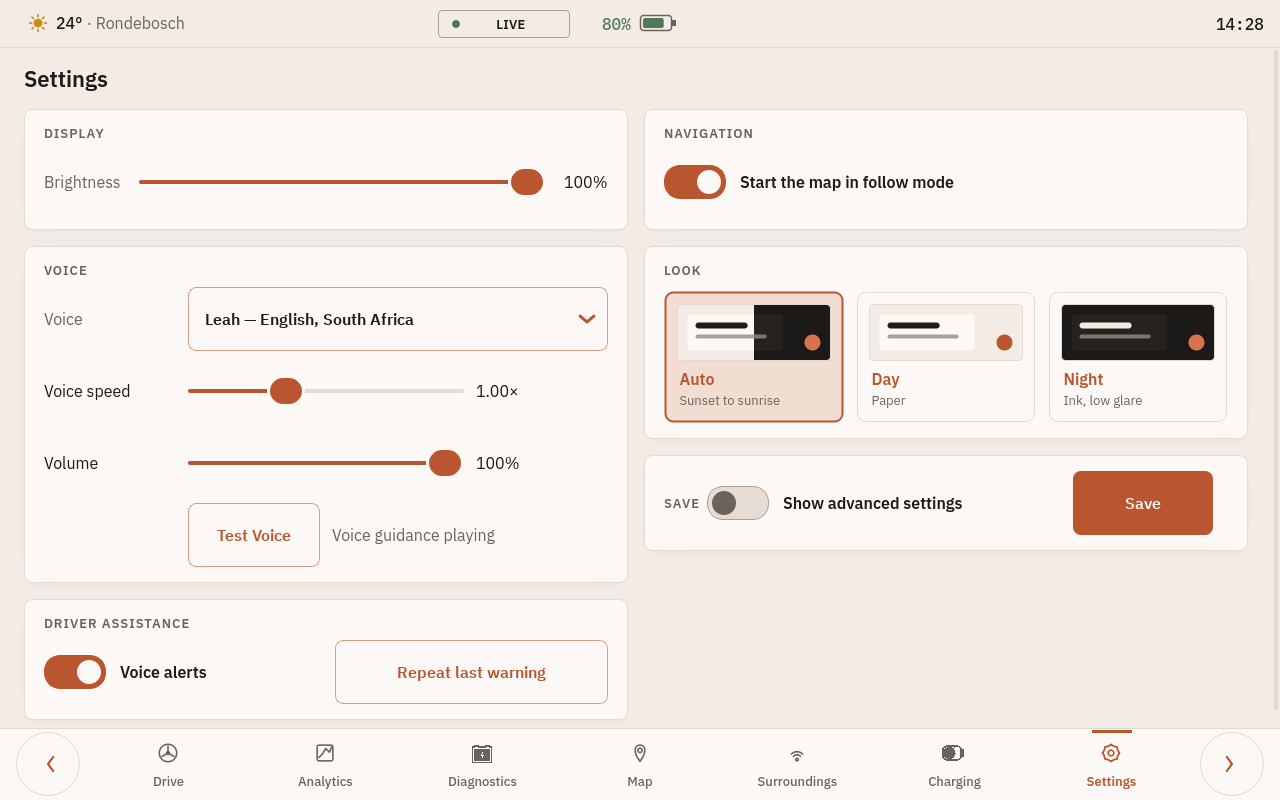
\includegraphics[width=0.48\textwidth]{figures/ui/ui_settings.png}}
\subfigure[Weather card, opened from the status bar.]{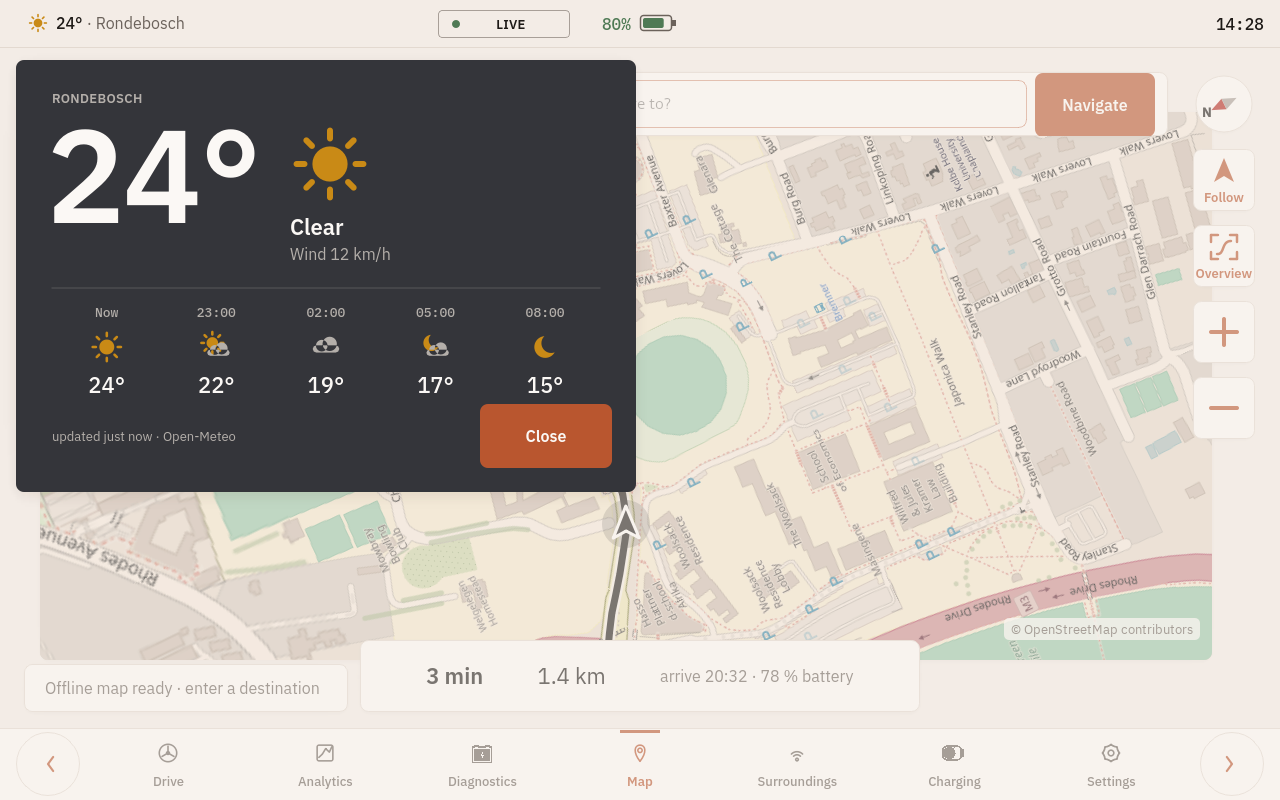
\includegraphics[width=0.48\textwidth]{figures/ui/ui_weather_card.png}}
\caption{Analytics, Settings and the weather card.}
\label{fig:ui-pages-b}
\end{figure}

\section{Verification}

The dashboard's test suite runs the patched application off screen against a copy of the team's source. It covers 14 test files:
\begin{itemize}
\item live data;
\item the map;
\item simulated-drive synchronisation;
\item search;
\item the analytics carousel;
\item the four layout tests;
\item the five style tests.
\end{itemize}

All passed on the final merged build on 12 October. The style tests check:
\begin{itemize}
\item the tap-colour and type-scale rules;
\item that the bundled fonts load;
\item that the weather item has no border or background;
\item every page in both themes, with no clipped labels;
\item that the battery animation runs.
\end{itemize}

Recorded widget trees and pixels show that the previous look is unchanged when the redesign is switched off. Paint times measured on the laptop were below 15\,ms per frame. The charging animation takes 1.0 to 1.5\,ms per frame, and runs only while its page is visible.

Two of the checks caught faults during the redesign:
\begin{itemize}
\item an off-screen test that reset the status bar's height hid the obstacle pill;
\item a test-cleanup step had been deleting the shared copy of the team's source between runs.
\end{itemize}

\outstanding{on the Raspberry Pi~5: paint times, touch response and the fonts on the panel; the 2\,s glance measurement on the vehicle; daylight contrast.}
